\section{Resultados e Discussão}

Simular gases de coulomb é especialmente interessante quando não há modelos de matrizes conhecidos, disponíveis ou simples para o $\Hf$ definido. Podemos, com a simulação de tais gases, calcular a média da função densidade das partículas, ou autovalores. Alternativamente, quando há modelos disponíveis em matrizes aleatórias essa medida poderia ser tirada diretamente do calculo de seus autovalores.

A família de ensembles gaussianos são modelos que mostramos ser bem representados como matrizes em \ref{Section: Ensembles Gaussianos}. Retorne os resultados da Seção \ref{Section: Potencias}. Tomar a medida dos ensembles gaussianos é o equivalente na simulação descrita a tomar 
\begin{equation}
d = 1; \ \  n = 2; \ \ \V(x)=\frac{|x|^2}{2}; \ \ W(x) = g(x) = \log{|x|}; \ \ \beta_N = \beta N^2; \ \ \beta = 1,2,4.
\label{Equation: Parametros Gaussian}
\end{equation}
O resultado da simulação para a configuração \ref{Equation: Parametros Gaussian} é apresentado na Figura \ref{Figura: Gaussian}. Apresentamos por contraste, na coluna da esquerda, os resultados para $N=10$, da densidade gerada pela simulação equivalente com matrizes para os três modelos ($\beta = 1,2,4$). Na coluna central, representa-se a comparação da simulação com o Semi-Círculo de Wigner, configuração de equilíbrio para os três modelos quando $N$ é grande o suficiente. Note que os valores foram escalados por $\sqrt{2 \beta}$ para melhor visualização. Finalmente, na coluna da direita apresentamos a distribuição do maior autovalor $\lambda_{max}$. Um resultado importante  \cite{Tracy} enuncia que existem $z_{N}^{(\beta)}$ e $s_N^{(\beta)}$ tais que $$\lim_{N \to \infty} \mathbb{P}_{\beta,N,V} \left( \frac{\lambda_{max} - z_{N}^{(\beta)}}{s_N^{(\beta)}} \leq x \right) = F_{\beta}(x),$$ onde $F_{\beta}(x)$ é a densidade acumulada de Tracy-Widow. Mostraremos a concordância desse resultado com a simulação na coluna da direita. Observa-se que os dois modelos à esquerda concordam bem na estimativa da medida para o $N$ usado. No centro, é possível notar que a medida de equilíbrio esperada, o Semi-Círculo de Wigner, é aproximada rapidamente pelo aumento de partículas no sistema. A distribuição do autovalor máximo é mais delicada, contudo, discordâncias em ordem de convergência são razoavelmente influentes na largura da curva e não são aparentes nos resultados.
\begin{figure}[ht!]
	\centering
	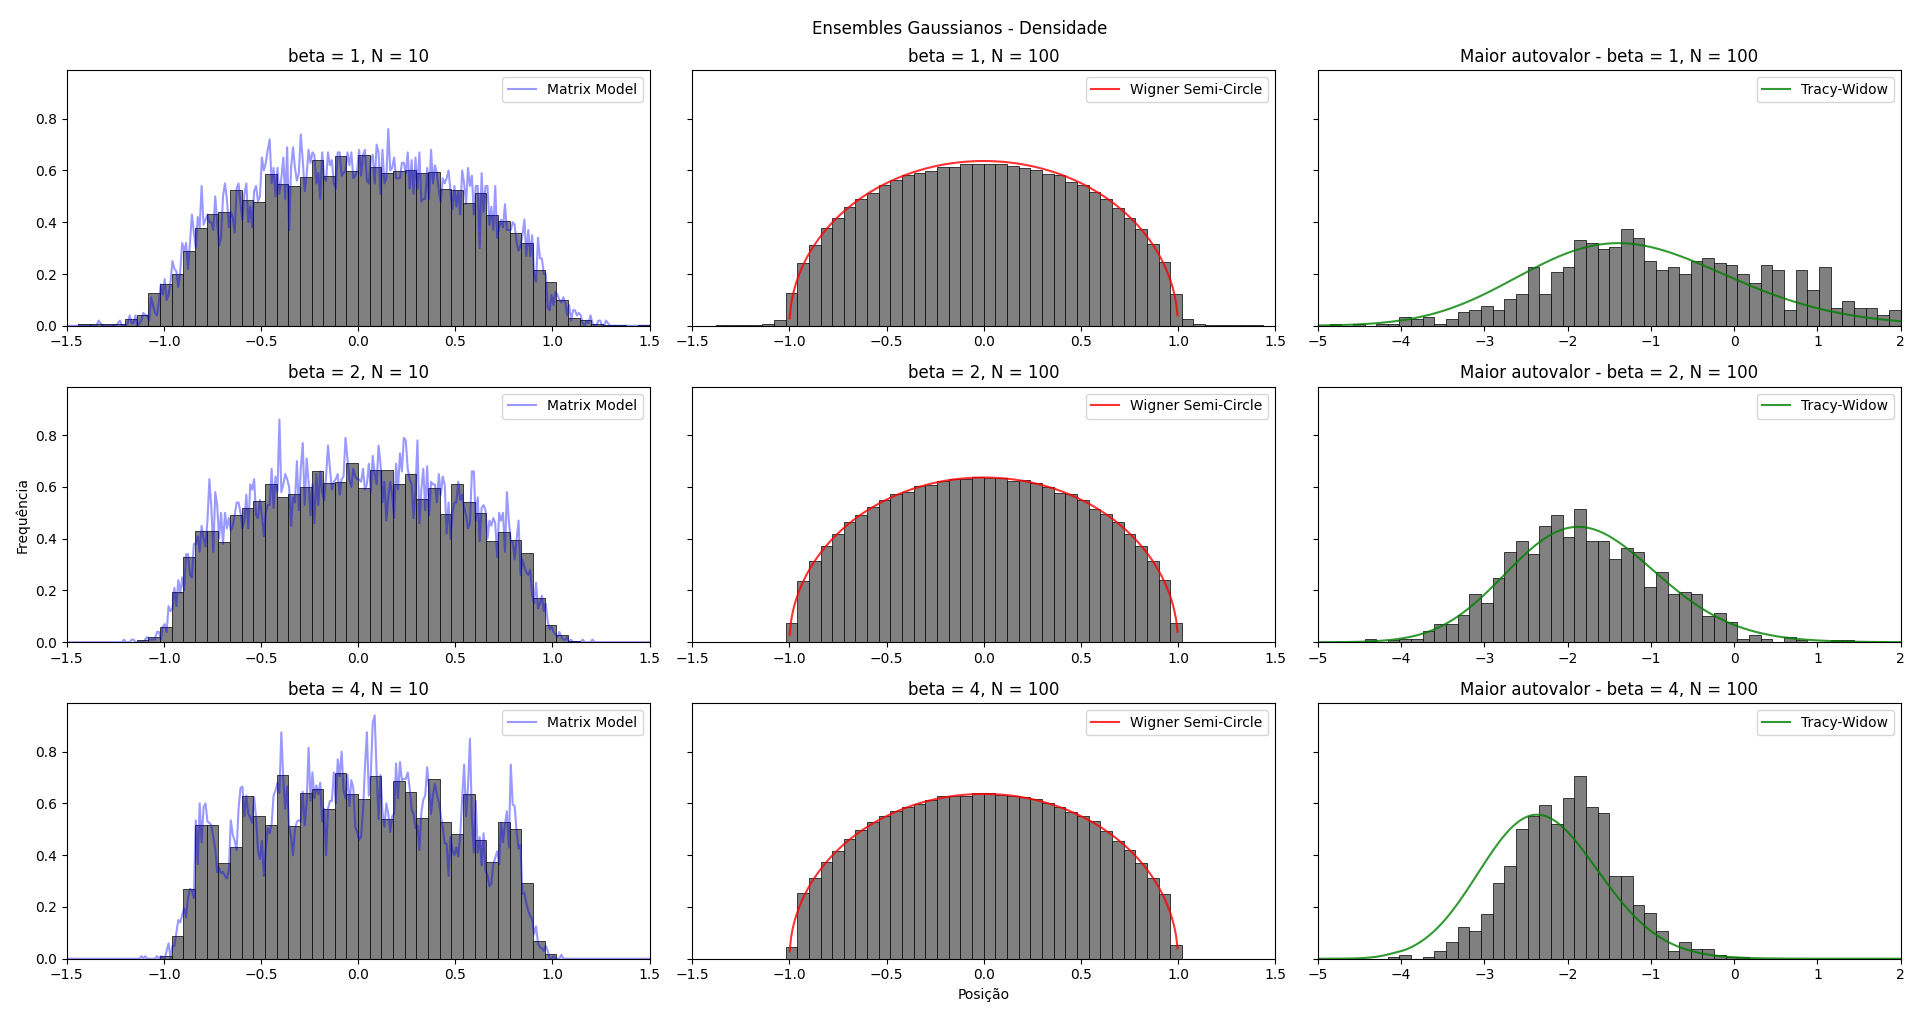
\includegraphics[width=0.95\textwidth]{Assets/validationGaussianTracy.png}
	\caption{Densidade para ensembles gaussianos, \ref{Equation: Parametros Gaussian}. Tomou-se $\Delta t = 0.5$ e $nsteps = 5\cdot10^6$ passos, registrando a cada $1000$ iterações a partir de $nsteps/5$. À esquerda da figura, em azul, a densidade da amostragem de $4\cdot10^3$ matrizes do ensemble. No centro, o Semi-Círculo de Wigner, medida de equilíbrio. Na direita, apresenta-se a densidade de $\lambda_{max}$ normalizado e sua mediada esperada.}
	\label{Figura: Gaussian}
\end{figure}

Podemos retomar também as descrições dos potenciais mônico em \ref{Equação: Mônico} e os dois regimes do potencial quártico, \ref{Equação: Quartico +} e \ref{Equação: Quartico -}. Respectivamente, estes modelos equivalem a tomar na simulação os parâmetros
\begin{equation}
	d = 1; \ \  n = 2; \ \ \V(x)= t |x|^{2m}; \ \ W(x) = g(x) = \log{|x|}; \ \ \beta_N = \beta N^2; \ \ \beta = 2.
	\label{Equation: Parametros Monico}
\end{equation}
\begin{equation}
	d = 1; \ \  n = 2; \ \ \V(x)=\frac{|x|^4}{4} + t \frac{|x|^2}{2}; \ \ W(x) = g(x) = \log{|x|}; \ \ \beta_N = \beta N^2; \ \ \beta = 2.
	\label{Equation: Parametros Quartico}
\end{equation}
O caso mônico se reduz ao gaussiano se $m=1$. Os resultados para ambos os potenciais estão explicitados na Figura \ref{Figura: Quartic Monic} para alguns parâmetros interessantes de $t$ e $m$.
\begin{figure}[ht!]
	\centering
	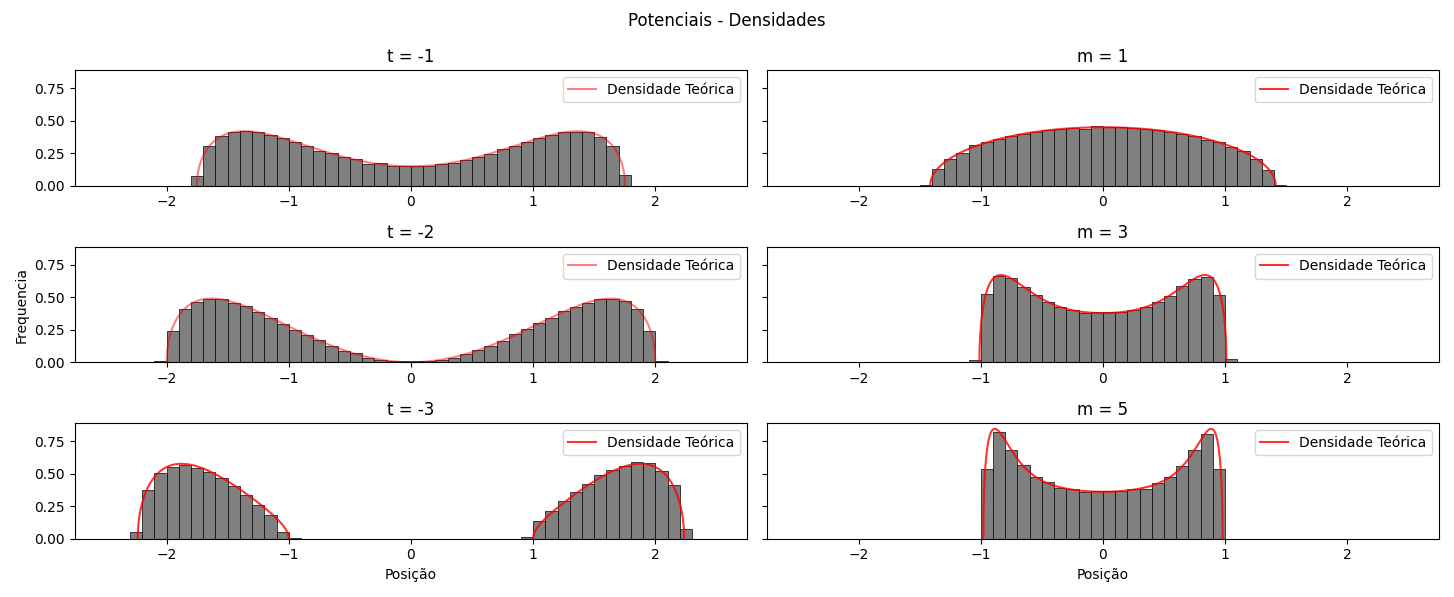
\includegraphics[width=0.95\textwidth]{Assets/validationQuarticMonic-alt.png}
	\caption{Potencial Quártico \ref{Equation: Parametros Quartico} e Mônico \ref{Equation: Parametros Monico}, respectivamente à esquerda e direita. Tomou-se $\Delta t = 0.1$, $N=100$, e $nsteps = 5\cdot10^6$ passos. Registra-se a cada $1000$ iterações a partir de $nsteps/5$. No Quártico, simula-se $t=-1,-2,-3$. No Mônico fixa-se $t=1$ e simula-se $m=1,3,5$.}
	\label{Figura: Quartic Monic}
\end{figure}

Novamente as medidas experimentais parecem convergir para a medida teórica enunciada em todas as configurações testadas. Contudo, isso é explorado e pode ser observado igualmente, com exceção do Mônico, em \cite{Chafa2018}. Em uma situação menos explorada, considere a seguinte configuração de potencial e autovalores complexos ($\R^d = \R^2$) e a representação das medidas simuladas para alguns valores de interesse de $t, a$ na Figura \ref{Figura: Complex},
\begin{equation}
	d = 2; \  n = 2; \  \V(z)=|z|^{2a} - \Re{t z^a};  \ W(x) = g(x) = \log{|x|};  \ \beta_N = \beta N^2;  \ \beta = 2.
	\label{Equation: Complex}
\end{equation}

\begin{figure}[ht]
	\centering
	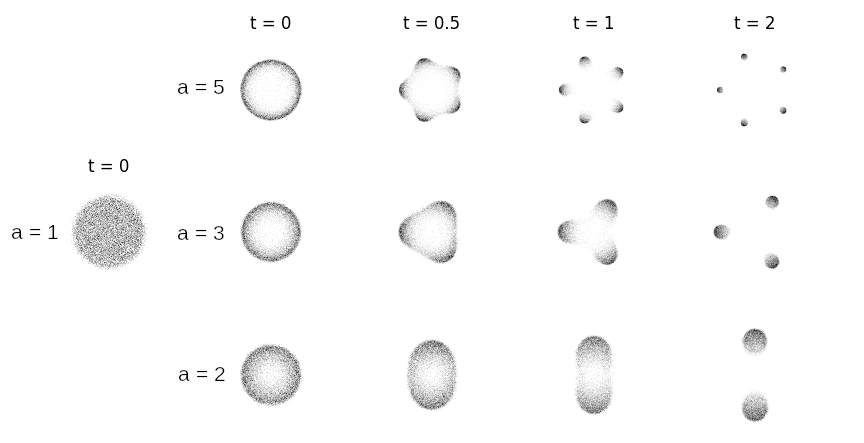
\includegraphics[width=\textwidth]{Assets/complexPotential.png}
	\caption{Medidas referentes à configuração \ref{Equation: Complex}. Tomou-se $\Delta t = 0.5$ e $nsteps = 2\cdot10^6$ passos, registrando a cada $500$ iterações a partir de $nsteps/5$.}
	\label{Figura: Complex}
\end{figure}

É previsto para esse modelo uma transição de regime, uma separação da medida de equilíbrio, para $t_c \approx \sqrt{\frac{1}{a}}$ \cite{balogh2016orthogonal}. A simulação replicar o comportamento esperado é um bom indicador de que é possível estudar a medida de tal ensemble numericamente, que pode ser explorado posteriormente. Outro fator que corrobora o bom comportamento do modelo é a medida uniforme quando $a=1$, também prevista pela teoria.

No Capítulo \ref{Capitulo: Intro} é notado que os modelos gaussianos são os únicos em RMT com invariância por rotação e independência das entradas simultaneamente. Gerar matrizes de outros modelos invariantes dependeria de gerar entradas correlacionadas ja que, se tratando de ensembles invariantes, ou seja, de medida igual para quaisquer $M, M'$ tais que $\matriz{M} = \matriz{U} \matriz{M'} \matriz{U}^{-1}$, podemos simular $\matriz{U}$ autovetores uniformemente do espaço correspondente. Isso pois sabemos do teorema espectral que, para as matrizes tomadas, vale a decomposição $\matriz{M} = \matriz{U} \matriz{D} \matriz{U}^{-1}$. Para reconstruir uma elemento do ensemble de interesse nos resta replicar a medida de autovalores, $\matriz{D}$. Isso, de forma interessante, pode ser feito pela simulação descrita de Gases de Coulomb, que replica a medida dos ensemble.

%Outra possibilidade interessante da replicação numérica dessas medidas é que, miniminizada a energia livre $E_{N, V}$, podemos fazer estimativas para constantes da expansão para $\log(Z_{\beta_N})$ proposta em trabalhos recentes, como em \cite{Byun_2023}. Essas estimativas podem dar uma ideia geral do comportamento dessas constantes, de relevante significado físico, para sistemas de interesse.  
